\section{Graphical representations.}

\subsection{Two-dimensional.}

We can represent any cubrix as a series of matrices separated by vertical bars, where each matrix would be a ``slice'' ($k=1$, $k=2$...) from the cubrix. This is the standard print representation.

\[ \left(
\begin{array}{c c c | c | c c c}
	\alpha_{111} & \cdots & \alpha_{1n1} &        & \alpha_{11o} & \cdots & \alpha_{1no} \\
	\vdots       &        & \vdots       & \cdots & \vdots       &        & \vdots       \\
	\alpha_{m11} & \cdots & \alpha_{mn1} &        & \alpha_{m1o} & \cdots & \alpha_{mno} \\
\end{array} \right)
\]

\subsection{Superficial three-dimensional.}

Sometimes it will suffice with a big-picture view of the cubrix which doesn't go into detail. For this purpose, we can organize each element in voxels which make up a rectangular prism.

\begin{figure}[H]
	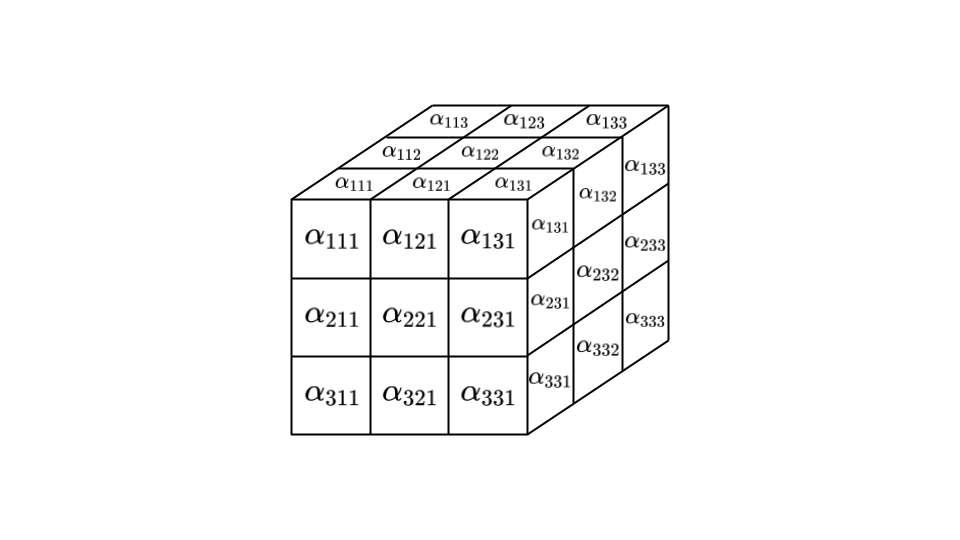
\includegraphics[width=\linewidth]{media/tridimensional_sup.png}
	\caption{Superficial three-dimensional representation of a cubrix with elements $\alpha_{ijk}$.}
\end{figure}

\newpage

\subsection{Complete three-dimensional.}

For a complete view which preserves the three-dimensional structure, we can separate each ``slice'' of the cubrix along a certain subindex. This representation can aid in pattern recognition.

\begin{figure}[H]
	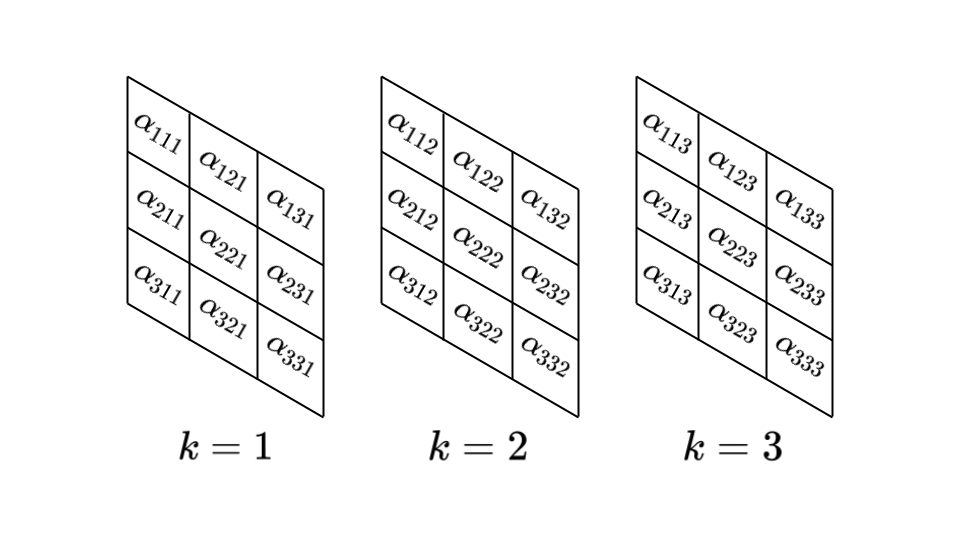
\includegraphics[width=\linewidth]{media/tridimensional_comp.png}
	\caption{Complete three-dimensional representation of a cubrix with elements $\alpha_{ijk}$.}
\end{figure}

\subsection{Product.}

Under the definition given, element $ijk$ of cubrix $\Delta = (AB\Gamma)$ will be equal to the product of $A$'s $i$th row by $B$'s $j$th column by $\Gamma$'s $k$th ``depth''.

\begin{figure}[H]
	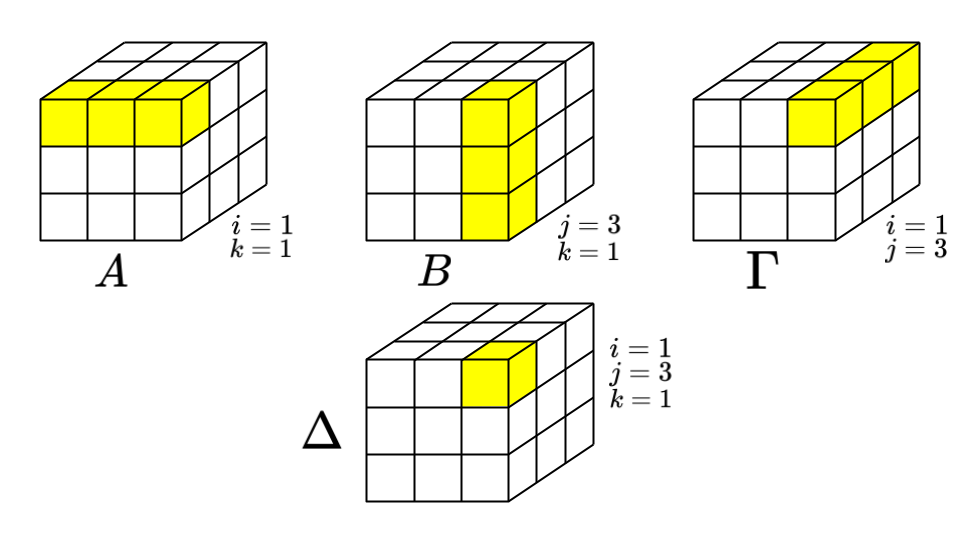
\includegraphics[width=\linewidth]{media/product.png}
	\caption{Superficial three-dimensional representation of the product $\Delta = (AB\Gamma)$.}
\end{figure}

This explains the restrictions marked by the cubrices' dimensions. In the sum's iterative process, it's necessary for the number of columns of $A$ ($n$) to equal the number of rows of $B$ ($p$) and to equal the number of ``depths'' of $\Gamma$ ($u$). Furthermore, $\Delta$ may not have more rows than $A$ nor than $\Gamma$ (otherwise, we would access non-existant values), nor more columns than $B$ or $\Gamma$, nor more ``depths'' than $A$ or $B$.
